\documentclass[a4,12pt]{horizon-theme}
\usepackage{lipsum}
\usepackage{fontawesome5}
\usepackage{graphicx,url}
\usepackage{float}
\usepackage{amsmath}
\usepackage{booktabs}
\usepackage{makecell}
\usepackage{array}
\usepackage{multirow}
\usepackage{caption}
\usepackage{subcaption}
\usepackage{siunitx}
\usepackage{enumerate}
\usepackage{gensymb}
\usepackage{csvsimple}
\usepackage{tabularray}
\usepackage{stackengine}
\usepackage{xcolor, colortbl}
\usepackage[round]{natbib}
\usepackage{karnaugh-map}
\usepackage{stackengine}
% \usepackage{longtable}
\usepackage{minted}
\usepackage{fontawesome}

\strutlongstacks{T}

\BeforeBeginEnvironment{minted}{\vspace{-20pt}}


% Cover Config
% \configCover{<num. do exp.>}{<data>}{<título>}
\configCover{P2}{14/07/2022}{Projeto de Relógio Digital}


\begin{filecontents*}{vcc1.csv}
pos,comp,vcc,gnd
C1,74190,16,8
C2,74190,16,8
C3,74190,16,8
C4,74190,16,8
C5,7411,14,7
C6,7402,14,7
C7,7411,14,7
C8,7402,14,7
\end{filecontents*}


\newenvironment{code}{\captionsetup{type=listing}}{}


\begin{document}
\horizonCover

\horizonTitle


\section{Introdução}
Uma FPGA é um circuito integrado criado para ser configurado por um projetista após sua fabricação com uma linguagem de descrição de hardware. Neste projeto, será usada uma FPGA na implementação da unidade de controle de um circuito digital de um relógio digital. Já o fluxo de dados será implementado utilizando circuitos integrados não programáveis (CIs TTL da família 74).

\section{Objetivos}
    O objetivo desse projeto consiste em projetar o circuito digital de um relógio com dois dígitos para os segundo e dois dígitos para os minutos. Além disso, o relógio deve ser programável e controlável.
    
\section{Planejamento}
\subsection{Descrição Funcional}
    O sistema digital em questão tem como principal função a contagem do tempo. Ele pode ser controlado por 5 sinais de controle (clock, Clear, Programa, Grava, Inibe) e possui dois modos de operação, o modo "Programação" (Programa = nível lógico "1") e o modo "Operação" (Programa = nível lógico "0"). 
    
    Quando no modo Programação, é possível configurar o valor de minutos e segundos desejados, basta ajustar os valores desejados na entrada de dados e colocar o sinal Grava em nível lógico "1", no clock seguinte o sinal de entrada será configurado na saída. O sinal Grava só possui efeito nesse modo de operação.
    
    Já o modo Operação funciona da seguinte maneira: se o sinal Inibe estiver em nível lógico baixo a saída contará o tempo a partir do valor de tempo configurado, caso contrário, se o sinal Inibe estiver em nível lógico alto, a contagem não ocorrerá. 
    
    O sinal clear zera as saídas no clock seguinte.


\subsection{Diagrama de Blocos}
    A Fig. \ref{fig:blocos} mostra o diagrama de blocos do circuito do relógio digital. O circuito recebe os sinais de controle clock, clear, programa, grava e inibe. Além disso, também recebe como entrada de dados 14 bits que correspondem aos valores de minutos e segundos a serem programados. Como saída, o circuito fornece 14 bits de dados que correspondem ao tempo atual que muda a cada clock, e sinais de depuração. A Unidade de Controle controla o Fluxo de Dados a partir dos sinais $\n{\textrm{c\_carrega}}$ e $\n{\textrm{c\_inibe}}$.

    \begin{figure}[!ht]
        \centering
        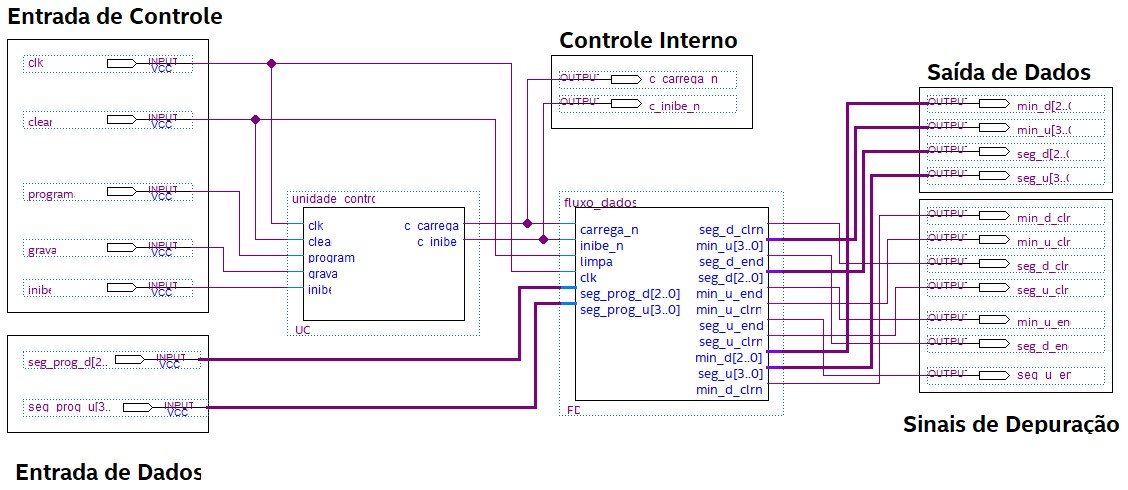
\includegraphics[width=1\textwidth]{diagrama_blocos.jpg}
        \caption{Diagrama de blocos do circuito do Relógio Digital}
        \label{fig:blocos}
    \end{figure}


\subsection{Diagrama Lógico}
    A Fig.\ref{fig:logico_fd} mostra a implementação do fluxo de dados utilizando-se 4 contadores 74190, 2 CIs de portas AND3 7411 e 2 CIs de portas NOR2 7411.
    
    \begin{figure}[!ht]
        \centering
        \stackinset{r}{1pt}{t}{1pt}{\carimboA{Relógio Digital}}{%
            \stackinset{l}{1pt}{b}{1pt}{\carimboB{vcc1.csv}}{%
                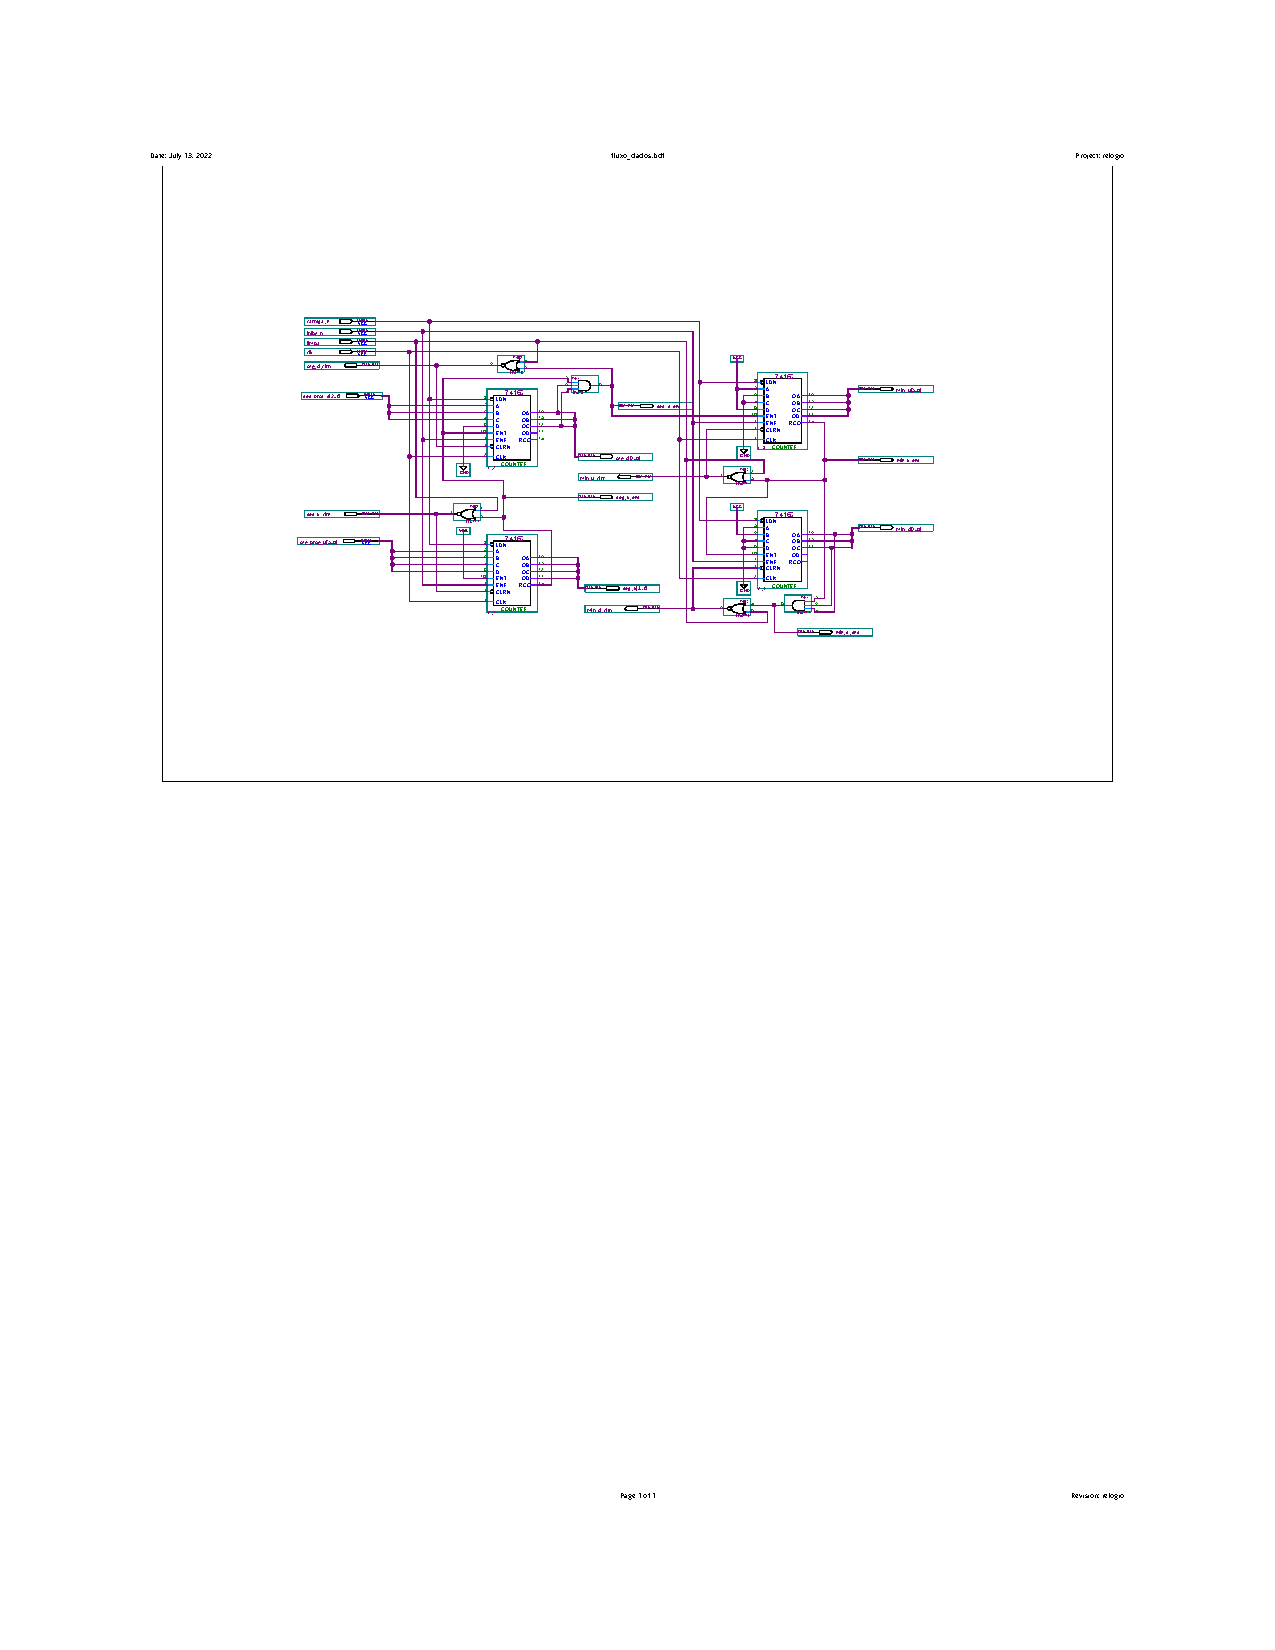
\includegraphics[width=\textwidth, trim={43mm, 165mm, 56mm, 45mm}, clip]{diagrama_logico.pdf}%
            }%
        }
        \caption{Diagrama lógico do Fluxo de Dados}
        \label{fig:logico_fd}
    \end{figure}


\newpage
\subsection{Diagrama de Estados}
A máquina de estados implementada na unidade de controle é composta por 3 estados, o primeiro consiste em um estado inicial do qual só se pode ir para o próximo estado que é o estado de programação onde o valor de minutos e segundos é carregado nos contadores do fluxo de dados, o outro estado é o de operação no qual o relógio começa a contar. Ao resetar o circuito, ele volta para o estado IDLE e só volta para o estado OP depois de passar pelo estado PROG. Isto é, o relógio só volta a contar depois de ser reprogramado.

\begin{figure}[!ht]
    \centering
    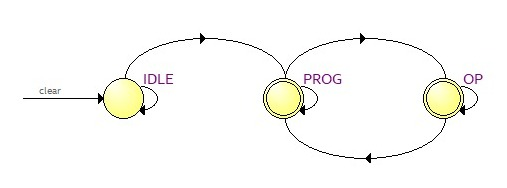
\includegraphics[width=\textwidth]{diagrama_estados.jpeg}
    \caption{Diagrama de estados da unidade de controle}
    \label{fig:estados}
\end{figure}

\newpage
\subsection{Simulação}

As Figs. \ref{fig:ct_fd}, \ref{fig:ct_uc} e \ref{fig:ct_completo} mostram as cartas de tempos da simulação do fluxo de dados, unidade de controle e ciruito completo, respectivamente.

\begin{figure}[!ht]
    \centering
    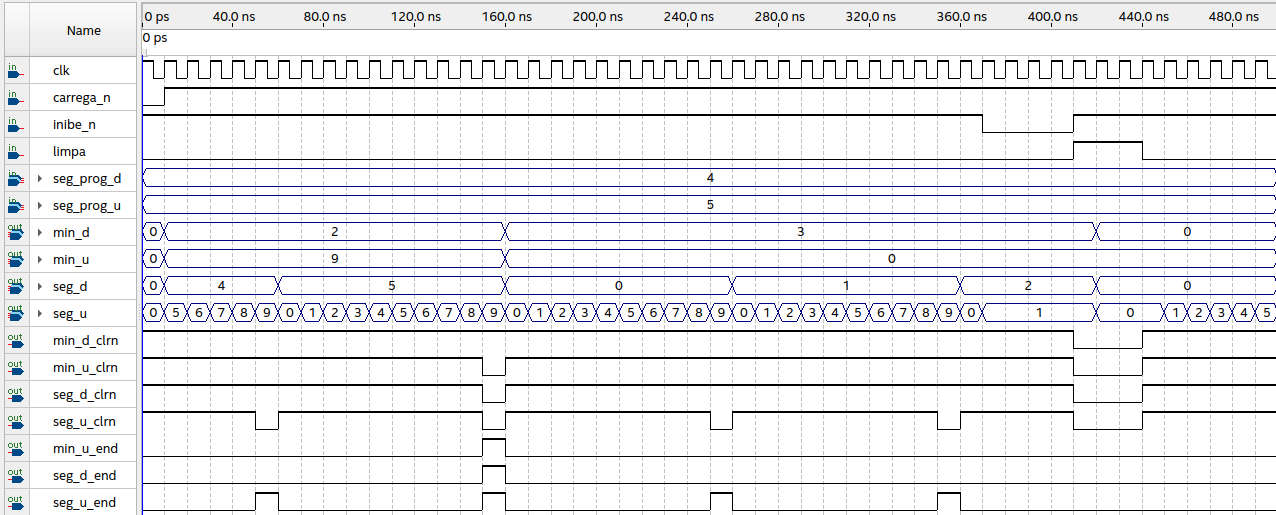
\includegraphics[width=\textwidth]{p2_fd.png}
    \caption{Carta de tempos do fluxo de dados}
    \label{fig:ct_fd}
\end{figure}

\begin{figure}[!ht]
    \centering
    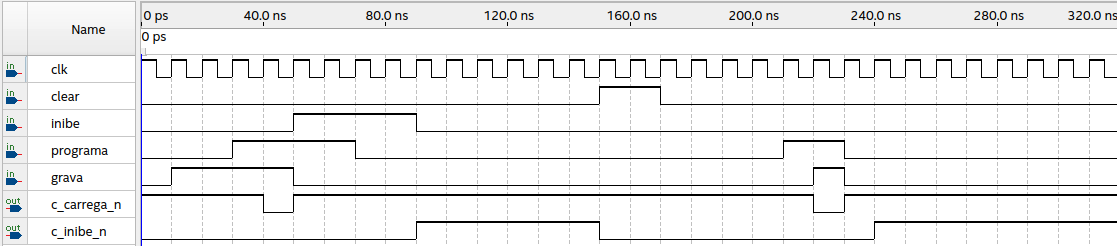
\includegraphics[width=\textwidth]{p2_uc.png}
    \caption{Carta de tempos da unidade de controle}
    \label{fig:ct_uc}
\end{figure}

\begin{figure}[!ht]
    \centering
    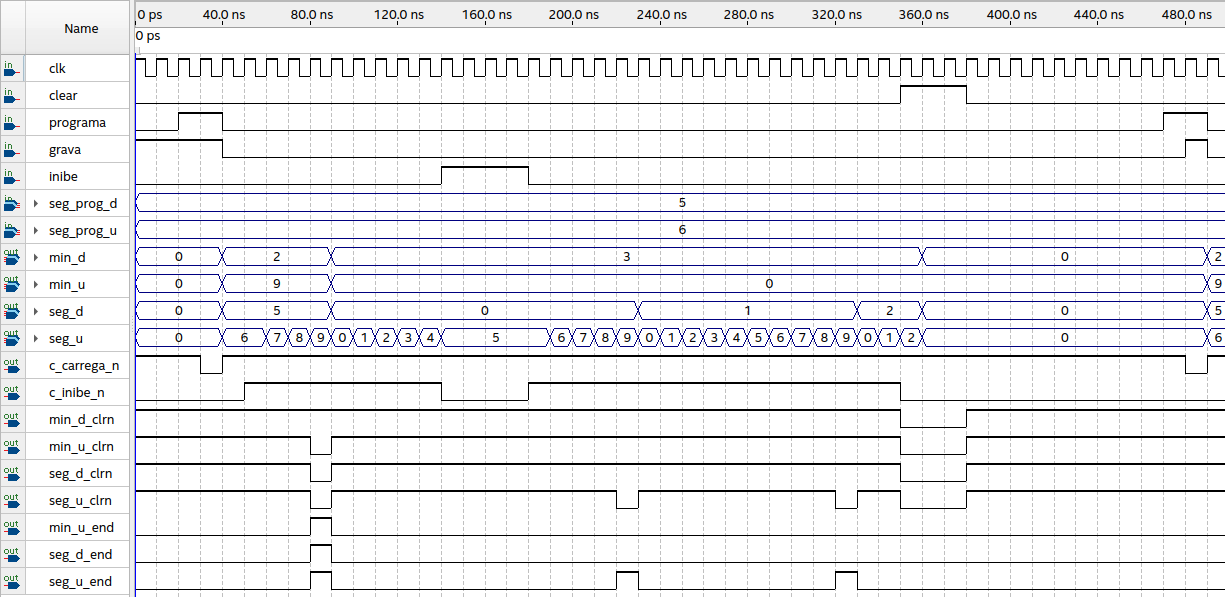
\includegraphics[width=\textwidth]{p2_completo.png}
    \caption{Carta de tempos do circuito completo}
    \label{fig:ct_completo}
\end{figure}

\newpage
\subsection{Testes}
As Tabelas \ref{tab:uc}, \ref{tab:fd} e \ref{tab:compelto} mostram as tabelas de testes da unidade de controle, do fluxo de dados e do circuito completo, respectivamente.

\begin{table}[!ht]
    \centering
    \caption{Tabela de testes da unidade de controle}
    \label{tab:uc}
    \doubleRuleSep
    \begin{tabular}{*{7}{c}}
        \doubleTopRule
        \multicolumn{5}{c}{Entradas} & \multicolumn{2}{c}{Saídas}\\
        \cmidrule(lr){1-5}\cmidrule(lr){6-7}
        clk & clear & inibe & programa & grava & c\_carrega\_n & c\_inibe\_n\\
        \midrule
        \csvreader[late after line=\\]{tb_uc.csv}{}%
        {\csvcoli & \csvcolii & \csvcoliii & \csvcoliv & \csvcolv & \csvcolvi & \csvcolvii}%
        \doubleBottomRule
    \end{tabular}
\end{table}

\begin{table}[!ht]
    \centering
    \caption{Tabela de testes do fluxo de dados com sinais os seguintes sinais: (1) clk, (2) clear, (3) carrega\_n, (4) inibe\_n, (5) seg\_prog\_d, (6) seg\_prog\_u, (7) min\_d, (8) min\_u, (9) seg\_d, (10) seg\_u, (11) min\_d\_clrn, (12) min\_u\_clrn, (13) seg\_d\_clrn, (14) seg\_u\_clrn, (15) min\_u\_end, (16) min\_d\_end, (17) seg\_u\_end}
    \label{tab:fd}
    \doubleRuleSep
    \begin{tabular}{*{17}{c}}
        \doubleTopRule
        \multicolumn{6}{c}{Entradas} & \multicolumn{4}{c}{Saídas} & \multicolumn{6}{c}{Depuração}\\
        \cmidrule(lr){1-6}\cmidrule(lr){7-10}\cmidrule(lr){11-17}
        1 & 2 & 3 & 4 & 5 & 6 & 7 & 8 & 9 & 10 & 11 & 12 & 13 & 14 & 15 & 16 & 17\\
        \midrule
        \csvreader[late after line=\\]{tb_fd.csv}{}%
        {\csvcolii & \csvcoliii & \csvcoliv & \csvcolv & \csvcolvi & \csvcolvii & \csvcolviii  & \csvcolix & \csvcolx & \csvcolxiii & \csvcolxiv & \csvcolxv & \csvcolxvi & \csvcolxvii & \csvcolxviii & \csvcolxix & \csvcolxx}%
        \doubleBottomRule
    \end{tabular}
\end{table}

\clearpage
\begin{table}[!ht]
    \centering
    \caption{Tabela de testes no circuito completo com os seguintes sinais: (1) clk, (2) clear, (3) programa, (4) grava, (5) inibe, (6) seg\_prog\_d, (7) seg\_prog\_u, (8) min\_d, (9) min\_u, (10) seg\_d, (11) seg\_u, (12) c\_carrega\_n, (13) c\_inibe\_n, (14) min\_d\_clrn, (15) min\_u\_clrn, (16) seg\_d\_clrn, (17) seg\_u\_clrn, (18) min\_u\_end, (19) min\_d\_end, (20) seg\_u\_end}
    \label{tab:completo}
    \doubleRuleSep
    \begin{tabular}{*{19}{c}}
        \doubleTopRule
        \multicolumn{7}{c}{Entradas} & \multicolumn{4}{c}{Saídas} & \multicolumn{8}{c}{Depuração}\\
        \cmidrule(lr){1-7}\cmidrule(lr){8-11}\cmidrule(lr){12-19}
        1 & 2 & 3 & 4 & 5 & 6 & 7 & 8 & 9 & 10 & 11 & 12 & 13 & 14 & 15 & 16 & 17 & 18 & 19\\
        \midrule
        \csvreader[late after line=\\]{tb_completo.csv}{}%
        {\csvcolii & \csvcoliii & \csvcoliv & \csvcolv & \csvcolvi & \csvcolvii & \csvcolviii  & \csvcolix & \csvcolx & \csvcolxi & \csvcolxii & \csvcolxiii & \csvcolxiv & \csvcolxv & \csvcolxvi & \csvcolxvii & \csvcolxviii & \csvcolxix & \csvcolxx }%
        \doubleBottomRule
    \end{tabular}
\end{table}



\subsection{Levantamento dos materiais necessários}
\label{sec:plan_materiais}
    
    \begin{table}[!ht]
        \centering
        \caption{Unidades requeridas para cada CI}
        \label{tab:materiais}
        \doubleRuleSep
        \begin{tabular}{lllrr}
            \doubleTopRule
            Slot & Operação & CI & Un. Requeridas & Un. Disponíveis \\
            \midrule
            1 & Contador & 74190 & 1 & 1\\
            2 & Contador & 74190 & 1 & 1\\
            3 & Contador & 74190 & 1 & 1\\
            4 & Contador & 74190 & 1 & 1\\
            5 & AND3 & 7411 & 1 & 2\\
            6 & OR2 & 7402 & 2 & 4\\
            7 & AND3 & 7411 & 1 & 2\\
            8 & OR2 & 7402 & 2 & 4\\
            \doubleBottomRule
        \end{tabular}
    \end{table}
    
    Para garantir que o circuito projetado respeite as restrições de montagem, fizemos um levantamento dos recursos necessários para este circuito mostrado na Tabela \ref{tab:materiais}. Ela mostra a quantidade de unidades lógicas requeridas para cada CI utilizado. As especificações de cada CI foi obtido pelos respectivos \emph{datasheets}.


\subsection{Montagem e Depuração}
\label{sec:montagem}

O circuito será montado e depurado por partes. A Tabela \ref{tab:sinais_fd} mostra a correlação dos sinais de depuração e dos LEDS da placa de montagem do fluxo de dados e a Tabela \ref{tab:sinais_uc} mostra a designação dos pinos da unidade de controle. Os sinais de saída (segundos e minutos) serão mostrados nos displays da placa de montagem. 

\begin{table}[!ht]  
    \centering
    \caption{Tabela de correlação dos sinais de depuração, entrada e saída com os LEDS, chaves e displays da placa de montagem do Fluxo de Dados}
    \label{tab:sinais_fd}
    \doubleRuleSep
    \begin{tabular}{cccc}
        \doubleTopRule
        Sinal & Endereço da Porta & LED/Display/Chave & Tipo E/S/D \\
        \midrule
        $Seg\_prog\_u[0]$ & 74162:1:3 & Chave 0 & Entrada\\
        $Seg\_prog\_u[1]$ & 74162:1:4 & Chave 1 & Entrada\\
        $Seg\_prog\_u[2]$ & 74162:1:5 & Chave 2 & Entrada\\
        $Seg\_prog\_u[3]$ & 74162:1:6 & Chave 3 & Entrada\\
        $Seg\_prog\_d[0]$ & 74162:2:3 & Chave 4 & Entrada\\
        $Seg\_prog\_d[1]$ & 74162:2:4 & Chave 5 & Entrada\\
        $Seg\_prog\_d[2]$ & 74162:2:5 & Chave 6 & Entrada\\
        $Seg\_u[0]$ & 74162:1:14 & Display D0:1 & Saída\\
        $Seg\_u[1]$ & 74162:1:13 & Display D0:2 & Saída\\
        $Seg\_u[2]$ & 74162:1:12 & Display D0:3 & Saída\\
        $Seg\_u[3]$ & 74162:1:11 & Display D0:4 & Saída\\
        $Seg\_d[0]$ & 74162:2:14 & Display D1:1 & Saída\\
        $Seg\_d[1]$ & 74162:2:13 & Display D1:2 & Saída\\
        $Seg\_d[2]$ & 74162:2:12 & Display D1:3 & Saída\\
        $Min\_u[0]$ & 74162:3:14 & Display D2:1 & Saída\\
        $Min\_u[1]$ & 74162:3:13 & Display D2:2 & Saída\\
        $Min\_u[2]$ & 74162:3:12 & Display D2:3 & Saída\\
        $Min\_u[3]$ & 74162:3:11 & Display D2:4 & Saída\\
        $Min\_d[0]$ & 74162:4:14 & Display D3:1 & Saída\\
        $Min\_d[1]$ & 74162:4:13 & Display D3:2 & Saída\\
        $Min\_d[2]$ & 74162:4:12 & Display D3:3 & Saída\\
        $Seg\_u\_clrn$ & 7402:1:1 & LED0 & Depuração\\
        $Seg\_d\_clrn$ & 7402:1:4 & LED1 & Depuração\\
        $Min\_u\_clrn$ & 7402:2:1 & LED2 & Depuração\\
        $Min\_d\_clrn$ & 7402:2:4 & LED3 & Depuração\\
        $Seg\_u\_end$ & 74162:1:15 & LED4 & Depuração\\
        $Seg\_d\_end$ & 7411:1:6 & LED5 & Depuração\\
        $Min\_u\_end$ & 74162:3:15 & LED6 & Depuração\\
        $Min\_d\_end$ & 7411:2:6 & LED7 & Depuração\\
        \doubleBottomRule
    \end{tabular}
\end{table}

\newpage
\begin{table}[!ht]
    \centering
    \caption{Tabela de designação de pinos da Unidade de Controle para a placa FPGA DE0-CV com Cyclone
V 5CEBA4F23C7}
    \label{tab:sinais_uc}
    \doubleRuleSep
    \begin{tabular}{rccc}
        \doubleTopRule
        % {} & \multicolumn{2}{c}{GPIO} & FPGA\\
        % \cmidrule(lr){2-3}\cmidrule(lr){4-4}
        Sinal & Código Interface & Código FPGA & Tipo E/C \\
        \midrule
        clk & GPIO\_0\_D0 & N16 & Entrada\\
        clear & GPIO\_0\_D4 & D17 & Entrada\\
        programa & GPIO\_0\_D5 & K20 & Entrada\\
        grava & GPIO\_0\_D6 & K21 & Entrada\\
        inibe & GPIO\_0\_D7 & K22 & Entrada\\
        $\n{\textrm{c\_carrega}}$ & GPIO\_1\_D4 & A13 & Controle\\
        $\n{\textrm{c\_inibe}}$ & GPIO\_1\_D5 & B13 & Controle\\
        \doubleBottomRule
    \end{tabular}
\end{table}



\section{Montagem e Resultados}
O fluxo de dados foi montado e testado por partes de acordo com a seguinte sequência seguinte sequência: (1) dezena de segundo; (2) dezena e unidade de segundo; (3) dezena de minuto e (4) dezena e unidade de minuto.

O objetivo dos teste das dezenas foi certificar a contagem de 0 a 5 e, durante a monagem e testes, as entradas dos CIs 74162 (contador) e 7411 (and) que dependiam do sinal RCO do dígito de unidade foram substituídos por VCC. Já o objetivo do teste dos dígitos de dezena e unidade foi testar a contagem de 0 a 60 com a devida sincronização dos dois dígitos.

Foi considerado o funcionamento correto da Unidade de Controle, já que ela havia passado por simulações e o circuito completo já havia sido construído e testado com sucesso em um open lab. Desta forma, os testes mensionados com o fluxo de dados foram feitos já com os sinais de controle provenientes da UC e os sinais externos (clock, reset, programa, grava e inibe) foram inseridos pelo Analog Discovery.

Não houve nenhum problema durante os testes individuais, apenas na execução do circuito completo foi detectado um teste com o sinal clear, na qual o dígito de unidade de minuto não estava sendo limpo. O problema foi resolvindo com a substituição do contador (CI 74162) por outro.

O circuito completo (Fig. \ref{ap:montagem}) foi testado de acordo com a Tabela \ref{tab:completo} com uma modificação do valor inicial do minuto para 59. Desta forma, foram testadas a troca de segundo, a troca de minuto e a troca de hora.

Além disso, não houve uso dos CI's conversores de tensão durante a montagem, pois o circuito já foi projetado para evitar o seu uso.


\section{Conclusão}
Neste experimento, um circuito de relógio digital foi projetado e implementado usando a separação em dois componentes: a Unidade de Controle e o Fluxo de Dados. O primeiro foi projetado em VHDL e implementado em uma FPGA Cyclone V e o segundo foi implementado no painel de montagens usando circuitos integrados TTL. O resultado da execução do circuito completo está condizente e satisfatória com relação às simulações. Além disso, a decisão de não usar conversores de tensão funcionou corretamente, já que poucos CI's foram utilizados e as ligações em série foram evitas, sendo substituídas por lugações em paralelo para evitar queda de tensão.

\clearpage
\newpage
\appendix
\section*{Apêndice}
\renewcommand{\thesubsection}{\Alph{subsection}}

\subsection{Descrições VHDL}
\label{ap:vhdl}

\begin{code}
\captionof{listing}{Descrição da Unidade de Controle}
\label{lst:uc}
\vspace{-12pt}
\inputminted[frame=lines, framesep=6pt, framerule=0.5pt, linenos, rulecolor=secondaryColor, breaklines]{VHDL}{unidade_controle.vhd}
\end{code}

\subsection{Montagem do circuito}
\label{ap:montagem}

\begin{figure}[!ht]
    \centering
    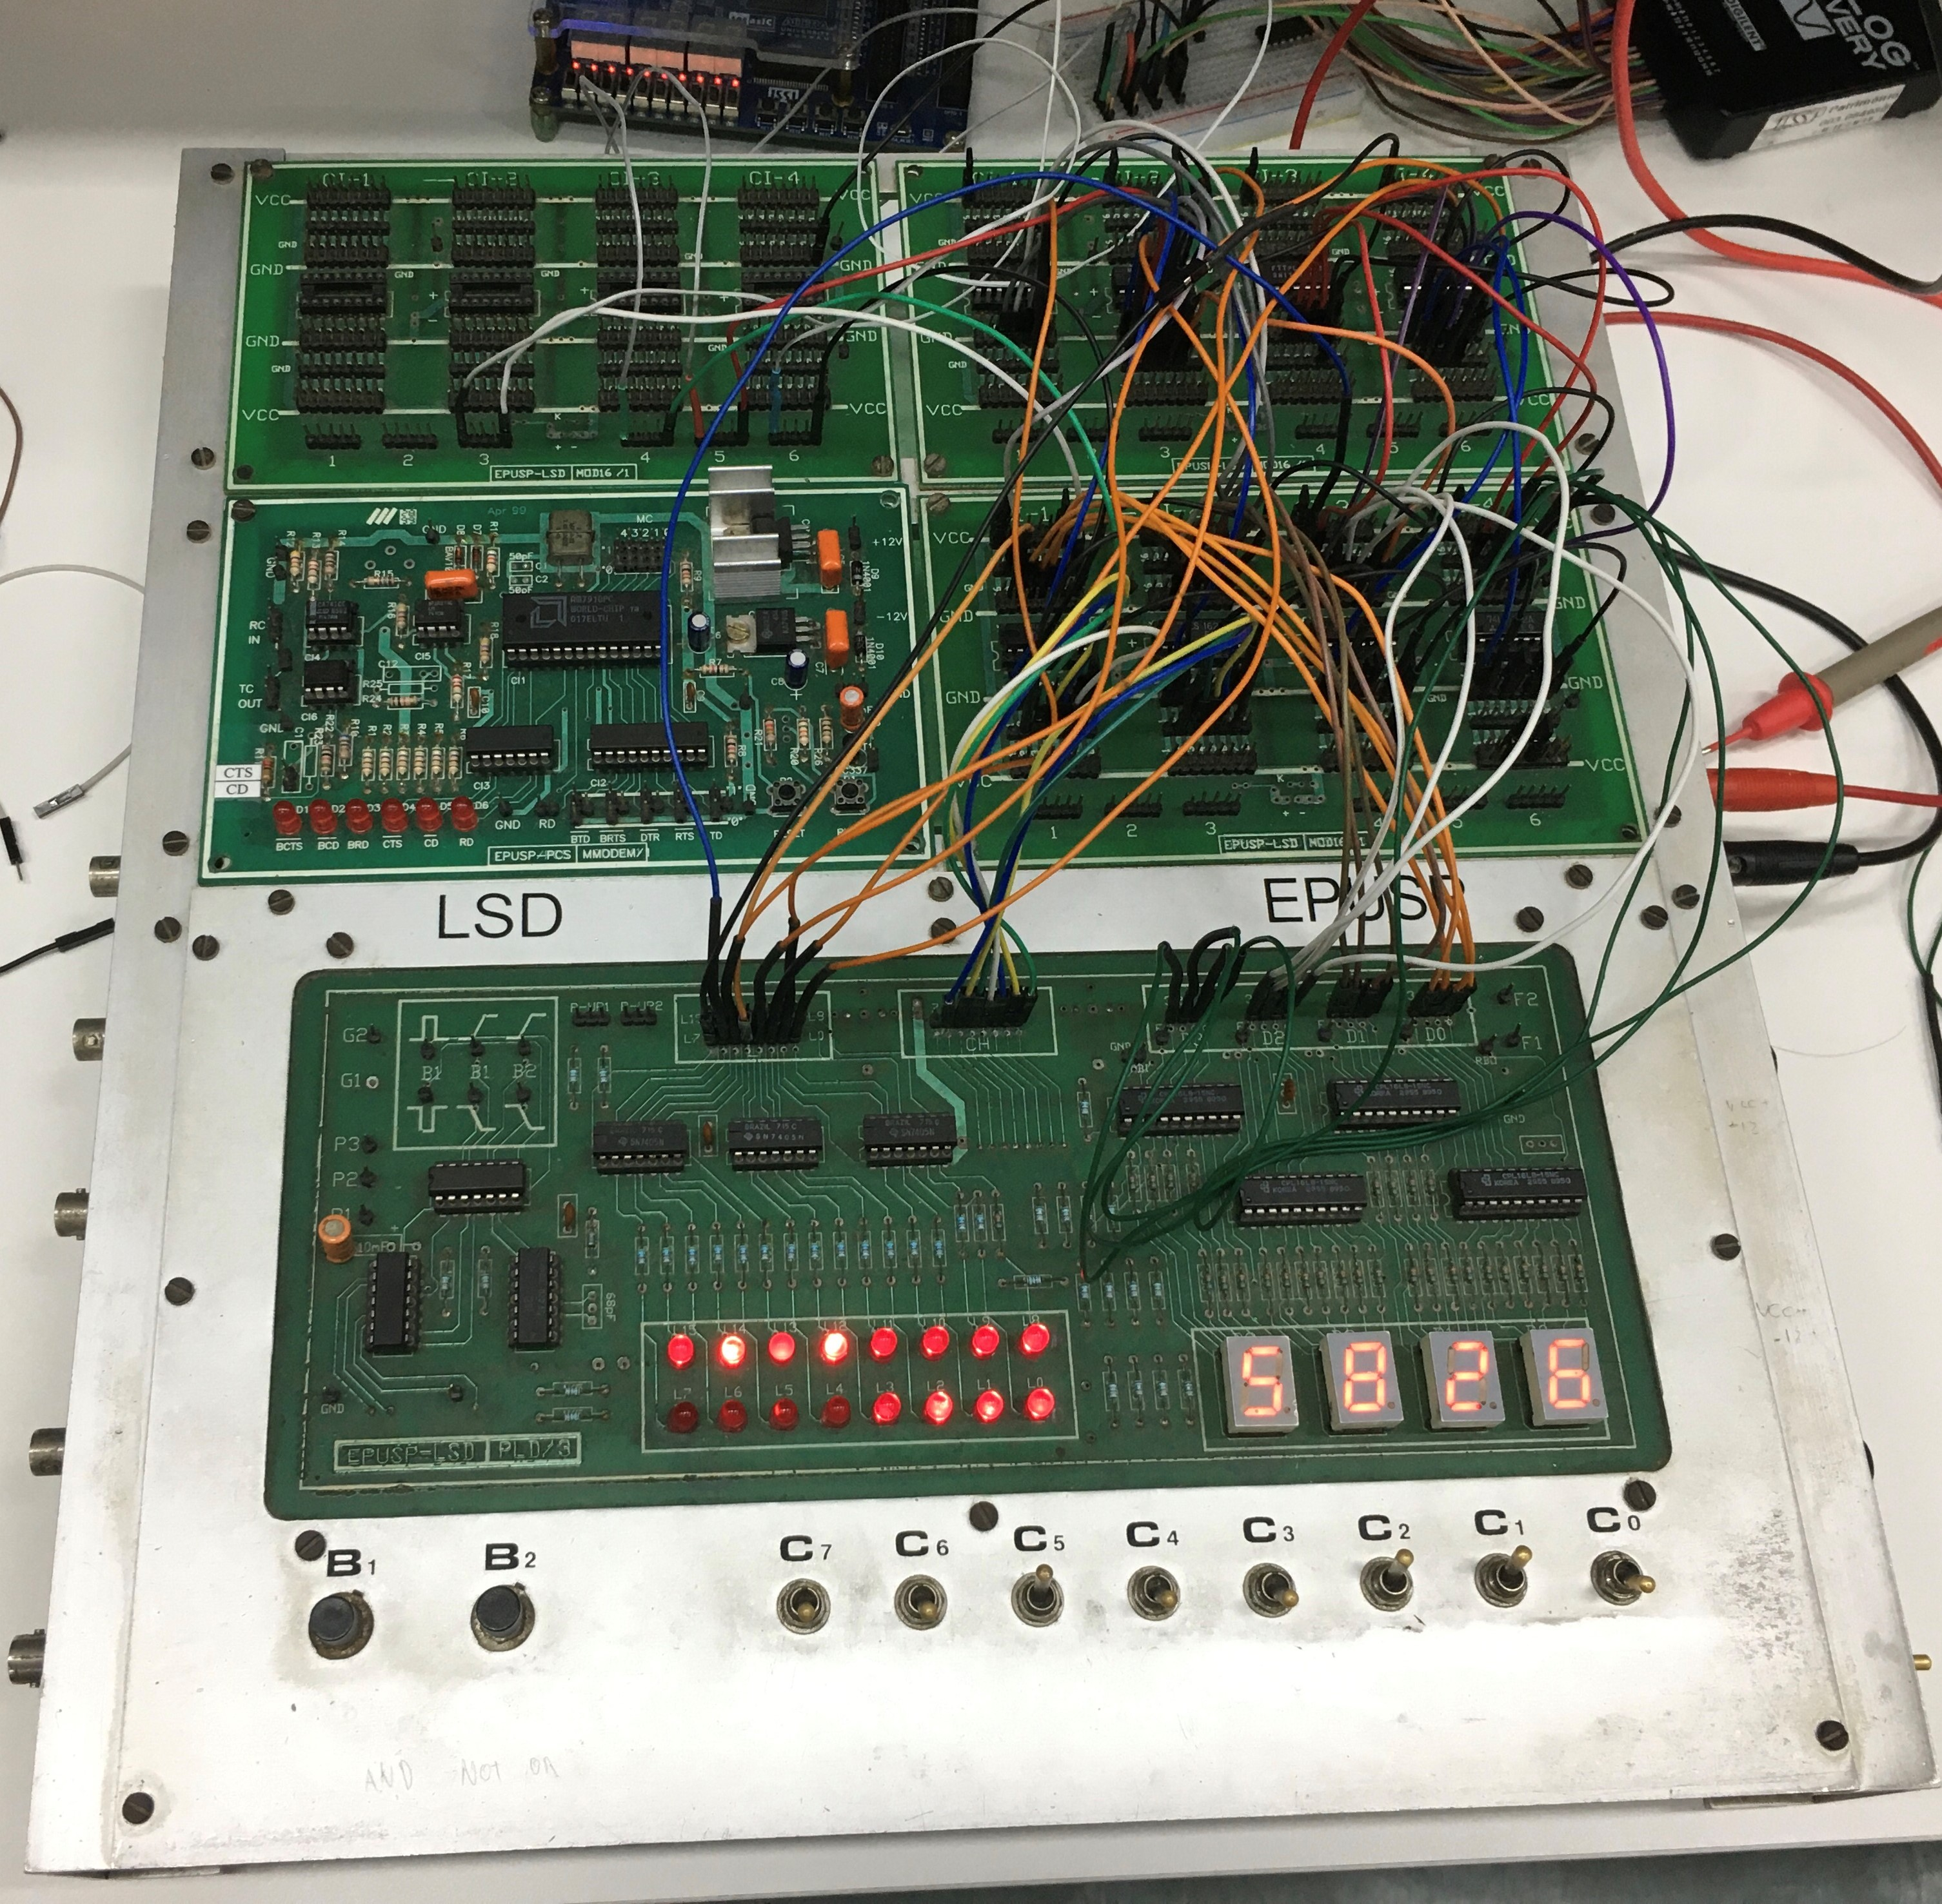
\includegraphics[width=\textwidth, trim={4cm 8cm 6cm 0}, clip]{montagem.jpg}
    \caption{Montagem do circuito completo}
    \label{fig:montagem}
\end{figure}

% \bibliographystyle{plainnat}
% \bibliography{refs}

\horizonBackCover
\end{document}